\documentclass[border=3pt]{standalone}
% Shared TikZ styles for the Ch. 3–8 diagrams (standalone PDFs); extends the Ch. 1 palette (s1_vs_llm_common.tex).
\usepackage[T1]{fontenc}
\usepackage{lmodern}
\usepackage[english]{babel}
\usepackage{amsmath,amssymb}
\usepackage{tikz}
\usetikzlibrary{shapes.geometric,shapes.misc,positioning,fit,arrows.meta,calc,backgrounds,decorations.pathreplacing,patterns}
\definecolor{ioFill}{HTML}{F1F0EC}\definecolor{ioLine}{HTML}{52514E}
\definecolor{modFill}{HTML}{E8F1FB}\definecolor{modLine}{HTML}{2A78D6}
\definecolor{decFill}{HTML}{ECE9F7}\definecolor{decLine}{HTML}{4A3AA7}
\definecolor{postFill}{HTML}{FFF6E0}\definecolor{postLine}{HTML}{EDA100}
\definecolor{okFill}{HTML}{EAF7F1}\definecolor{okLine}{HTML}{1BAF7A}
\definecolor{badFill}{HTML}{FDECEC}\definecolor{badLine}{HTML}{E34948}
\definecolor{nmFill}{HTML}{EFEAF8}\definecolor{nmLine}{HTML}{4A3AA7}
\definecolor{loopRed}{HTML}{E34948}\definecolor{clusterLine}{HTML}{9A9890}\definecolor{ink2}{HTML}{52514E}
\definecolor{orangeA}{HTML}{EB6834}
\tikzset{
  every node/.style={font=\small, align=center},
  io/.style={trapezium, trapezium left angle=72, trapezium right angle=108, trapezium stretches body,
             draw=ioLine, fill=ioFill, thick, inner sep=3pt, minimum height=2.4em},
  model/.style={rectangle, draw=modLine, fill=modFill, very thick, inner sep=4pt, minimum height=2.4em, text width=#1},
  model/.default=3.6cm,
  post/.style={rectangle, draw=postLine, fill=postFill, very thick, inner sep=4pt, minimum height=2.2em, text width=#1},
  post/.default=3.6cm,
  data/.style={cylinder, shape border rotate=90, aspect=0.18, draw=okLine, fill=okFill, very thick, inner sep=3pt, minimum height=2.6em, text width=#1},
  data/.default=2.4cm,
  decision/.style={diamond, aspect=2.1, draw=decLine, fill=decFill, very thick, inner sep=1pt},
  outcome/.style={rounded rectangle, draw=#1, thick, inner sep=4pt, minimum height=2em},
  arrow/.style={-{Latex[length=2mm]}, thick, ioLine},
  dashedarrow/.style={-{Latex[length=2mm]}, thick, ioLine, dashed},
  loop/.style={-{Latex[length=2.4mm]}, line width=1.4pt, loopRed},
  cluster/.style={draw=clusterLine, dashed, rounded corners=3pt, inner sep=7pt},
  clusterlabel/.style={font=\small\bfseries, text=ioLine},
  note/.style={font=\footnotesize, text=ink2},
  tok/.style={rectangle, draw=ioLine, fill=ioFill, thin, inner sep=2pt, minimum height=1.6em, font=\footnotesize},
  vmark/.style={rectangle, draw=orangeA, fill=postFill, thick, inner sep=2pt, minimum height=1.6em, font=\footnotesize\ttfamily},
}

\begin{document}
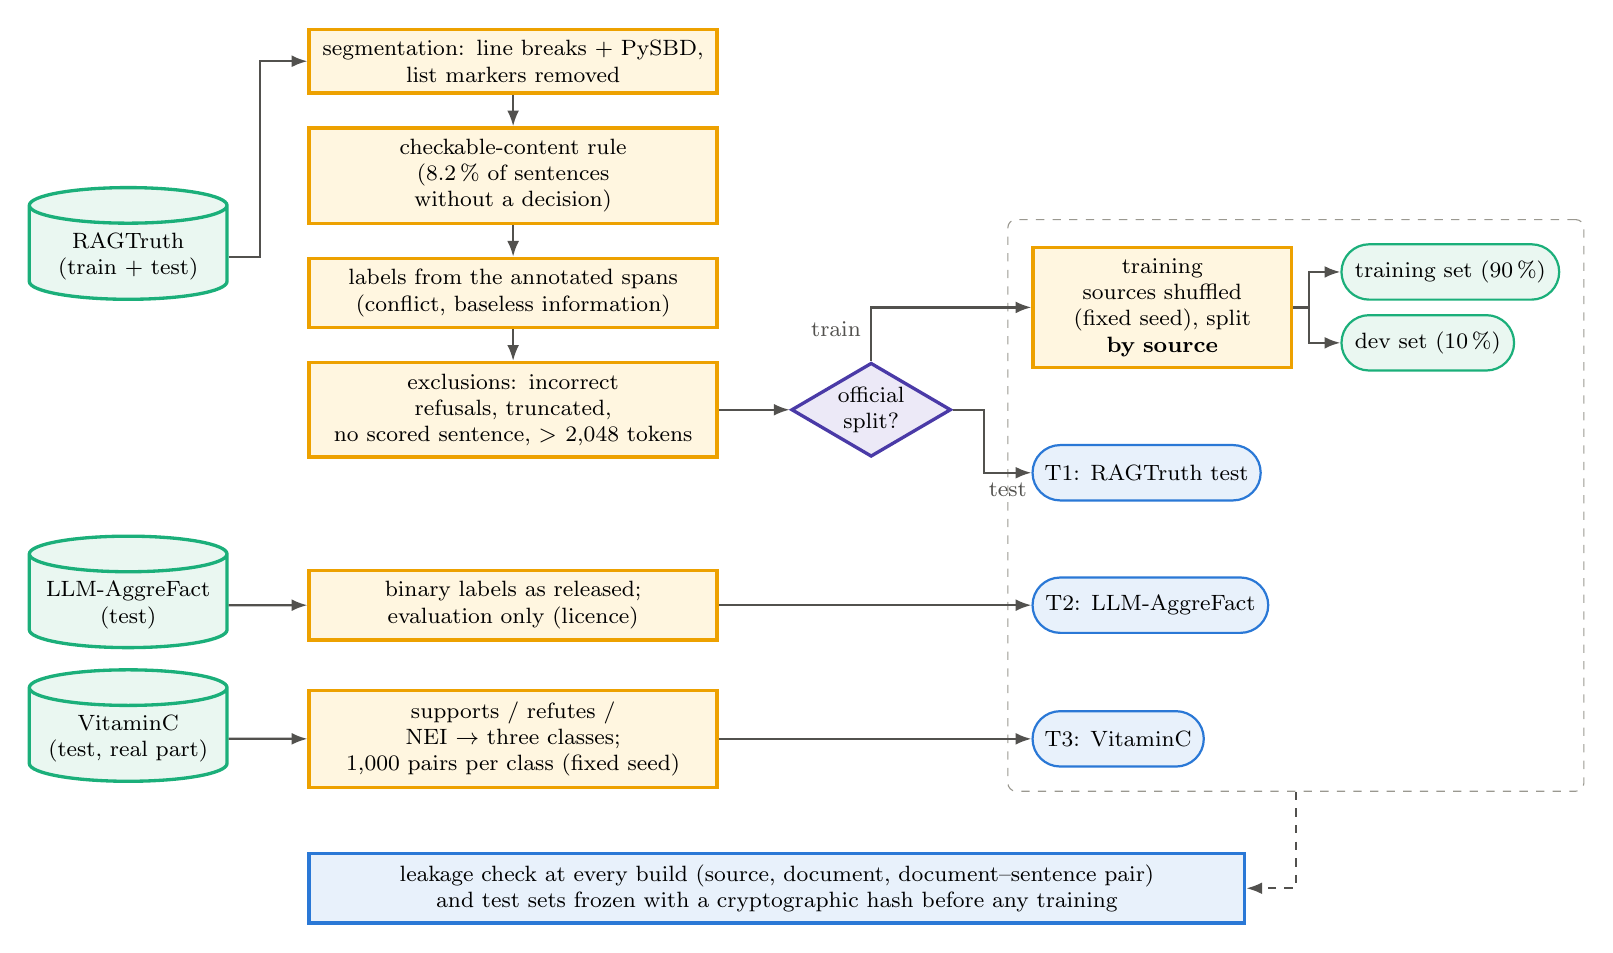
\begin{tikzpicture}[node distance=4mm]
  % column 2: RAGTruth processing chain
  \node[post=4.9cm, font=\footnotesize] (seg) at (0,0) {segmentation: line breaks + PySBD,\\list markers removed};
  \node[post=4.9cm, below=of seg, font=\footnotesize] (chk) {checkable-content rule\\(8.2\,\% of sentences without a decision)};
  \node[post=4.9cm, below=of chk, font=\footnotesize] (lab) {labels from the annotated spans\\(conflict, baseless information)};
  \node[post=4.9cm, below=of lab, font=\footnotesize] (exc) {exclusions: incorrect refusals, truncated,\\no scored sentence, $> 2{,}048$ tokens};
  \foreach \a/\b in {seg/chk,chk/lab,lab/exc} \draw[arrow] (\a) -- (\b);
  % column 1: sources
  \node[data=2.3cm, font=\footnotesize, left=10mm of lab.north west, anchor=east] (rt) {RAGTruth\\(train + test)};
  \draw[arrow] (rt.east) -- ++(4mm,0) |- (seg.west);
  % column 3: splits
  \node[decision, font=\footnotesize, aspect=1.7, right=9mm of exc] (spl) {official\\split?};
  \draw[arrow] (exc) -- (spl);
  \node[post=3.0cm, font=\footnotesize, right=10mm of spl, yshift=13mm] (src) {training sources shuffled\\(fixed seed), split\\\textbf{by source}};
  \node[outcome=okLine, fill=okFill, font=\footnotesize, right=6mm of src, yshift=4.5mm] (tr) {training set (90\,\%)};
  \node[outcome=okLine, fill=okFill, font=\footnotesize, right=6mm of src, yshift=-4.5mm] (dv) {dev set (10\,\%)};
  \node[outcome=modLine, fill=modFill, font=\footnotesize, anchor=west] (t1) at ([xshift=10mm, yshift=-8mm]spl.east) {T1: RAGTruth test};
  \draw[arrow] (spl.north) |- node[pos=0.3, left, font=\footnotesize] {train} (src.west);
  \draw[arrow] (spl.east) -- ++(4mm,0) |- node[pos=0.75, below, font=\footnotesize] {test} (t1.west);
  \draw[arrow] (src.east) -- ++(2mm,0) |- (tr.west); \draw[arrow] (src.east) -- ++(2mm,0) |- (dv.west);
  % other sources
  \node[post=4.9cm, font=\footnotesize, below=14mm of exc] (afp) {binary labels as released;\\evaluation only (licence)};
  \node[data=2.3cm, font=\footnotesize] (af) at (rt |- afp) {LLM-AggreFact\\(test)};
  \node[outcome=modLine, fill=modFill, font=\footnotesize, anchor=west] (t2) at (t1.west |- afp) {T2: LLM-AggreFact};
  \node[post=4.9cm, font=\footnotesize, below=6mm of afp] (vcp) {supports / refutes / NEI $\rightarrow$ three classes;\\1{,}000 pairs per class (fixed seed)};
  \node[data=2.3cm, font=\footnotesize] (vc) at (rt |- vcp) {VitaminC\\(test, real part)};
  \node[outcome=modLine, fill=modFill, font=\footnotesize, anchor=west] (t3) at (t1.west |- vcp) {T3: VitaminC};
  \draw[arrow] (af) -- (afp); \draw[arrow] (afp) -- (t2);
  \draw[arrow] (vc) -- (vcp); \draw[arrow] (vcp) -- (t3);
  % checks
  \node[model=11.6cm, font=\footnotesize, below=8mm of vcp.south west, anchor=north west] (lk) {leakage check at every build (source, document, document--sentence pair)\\and test sets frozen with a cryptographic hash before any training};
  \begin{scope}[on background layer]
    \node[cluster, fit=(tr)(dv)(t1)(t2)(t3)(src), inner sep=3mm] (outs) {};
  \end{scope}
  \draw[dashedarrow] (outs.south) |- (lk.east);
\end{tikzpicture}
\end{document}
